\documentclass{beamer}
\usetheme{Hannover}
\setbeamersize{sidebar width left=0pt}
\usepackage[T1, T2A]{fontenc}
\usepackage[utf8]{inputenc}
\usepackage[russian]{babel}
\usepackage{hyperref}
\usepackage{graphicx}
\graphicspath{ {../Images/} }

\author{Григорий Матюхин}
\date{\today}
\title{Лабораторная работа \textnumero13.}
\subtitle{Фильтр пакетов}

\begin{document}
\begin{frame}[plain]
	\titlepage
\end{frame}
\section{Цель работы}
\begin{frame}[plain]
	\frametitle{Цель работы}
	Получить навыки настройки пакетного фильтра в Linux.
\end{frame}

\subsection{Управление брандмауэром с помощью \texttt{firewall-cmd}}
\begin{enumerate}
	\begin{frame}[plain]
		\frametitle{Управление брандмауэром с помощью \texttt{firewall-cmd}}
		\item Определите текущую зону по умолчанию:
		\item Определите доступные зоны:
		\\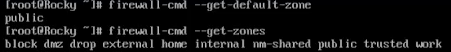
\includegraphics{1.png}
	\end{frame}
	\begin{frame}[plain]
		\item Посмотрите службы, доступные на вашем компьютере:
		\\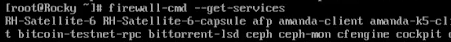
\includegraphics{2.png}
	\end{frame}
	\begin{frame}[plain]
		\item Определите доступные службы в текущей зоне:
		\\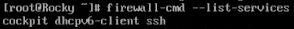
\includegraphics{3.png}
	\end{frame}
	\begin{frame}[plain]
		\item Сравните результаты вывода информации при использовании команды
		\texttt{firewall-cmd --list-all}
		и команды
		\texttt{firewall-cmd --list-all --zone=public}:
		\\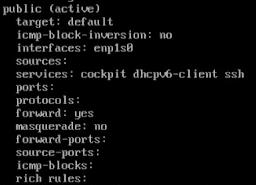
\includegraphics{4.png}
	\end{frame}
	\begin{frame}[plain]
		\item Добавьте сервер VNC в конфигурацию брандмауэра:
		\\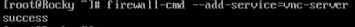
\includegraphics{5.png}
	\end{frame}
	\begin{frame}[plain]
		\item Проверьте, добавился ли vnc-server в конфигурацию:
		\\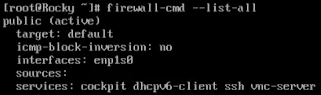
\includegraphics{6.png}
	\end{frame}
	\begin{frame}[plain]
		\item Перезапустите службу firewalld:
		\item Проверьте, есть ли vnc-server в конфигурации:
		\\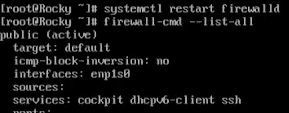
\includegraphics{7.png}
	\end{frame}
	\begin{frame}[plain]
		\item Добавьте службу vnc-server ещё раз, но на этот раз сделайте её постоянной
		\item Поверьте наличие \texttt{vnc-server} в конфигурации:
		\\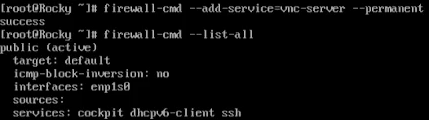
\includegraphics{8.png}
	\end{frame}
	\begin{frame}[plain]
		\item Перезагрузите конфигурацию \texttt{firewalld} и просмотрите конфигурацию времени выполнения:
		\\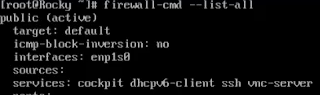
\includegraphics{9.png}
	\end{frame}
	\begin{frame}[plain]
		\item Добавьте в конфигурацию межсетевого экрана порт 2022 протокола TCP:
		\\
\includegraphics{10.png}
	\end{frame}
	\begin{frame}[plain]
		\item Проверьте, что порт добавлен в конфигурацию:
		\\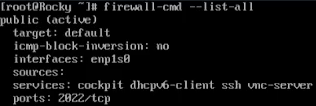
\includegraphics{11.png}
	\end{frame}
\end{enumerate}

\subsection{Управление брандмауэром с помощью \texttt{firewall-config}}
\begin{frame}[plain]
	\frametitle{Управление брандмауэром с помощью \texttt{firewall-config}}
	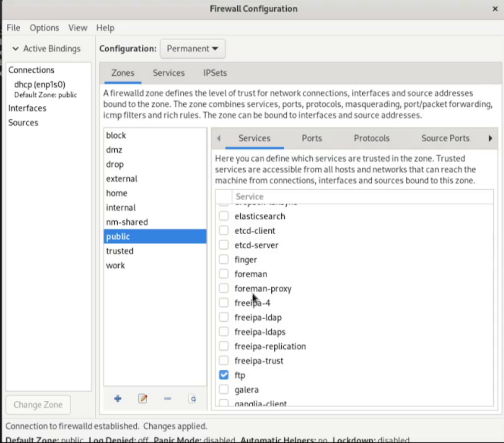
\includegraphics{12.png}
\end{frame}
\begin{frame}[plain]
	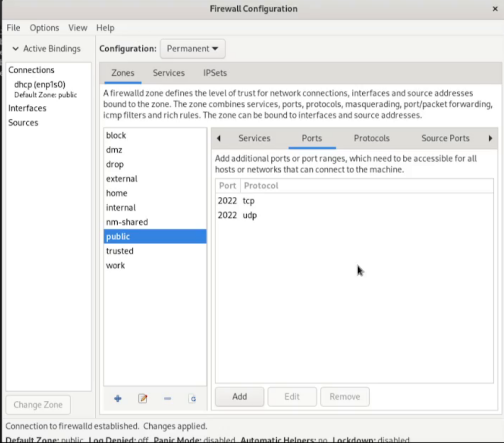
\includegraphics{13.png}
\end{frame}
\begin{frame}[plain]
	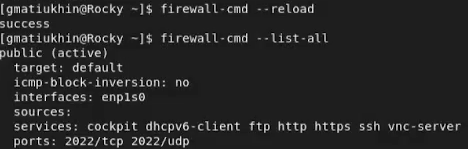
\includegraphics{14.png}
\end{frame}

\subsection{Самостоятельная работа}
\begin{frame}[plain]
	\frametitle{Самостоятельная работа}
	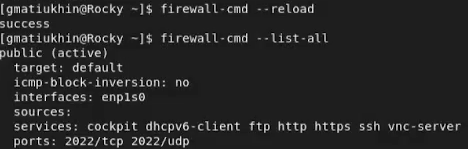
\includegraphics{14.png}
\end{frame}
\begin{frame}[plain]
	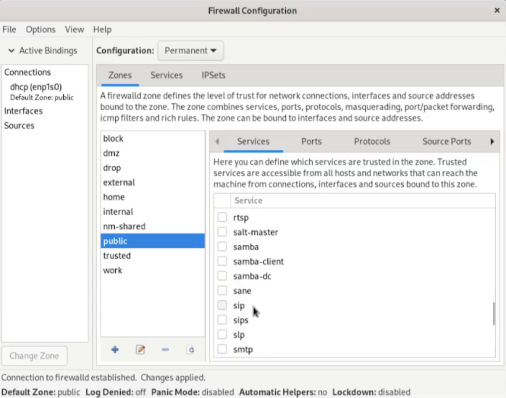
\includegraphics{16.png}
\end{frame}
\begin{frame}[plain]
	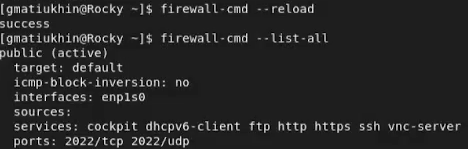
\includegraphics{14.png}
\end{frame}
\begin{frame}[plain]
	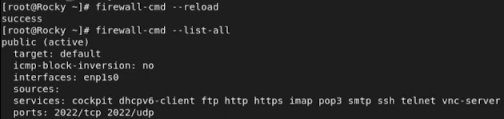
\includegraphics{17.png}
\end{frame}

\section{Вывод}
\begin{frame}[plain]
	\frametitle{Вывод}
	В ходе выполнения данной работы я получил навыки настройки пакетного фильтра в Linux.
\end{frame}

\end{document}
